\chapter{Implementation}
\label{chp:implementation} 

\section{Introduction}

This chapter presents four implementations that were developed during this project:

\begin{center}
	\begin{tabular}{ l p{7cm} }
	\textbf{Robot software in \ac{ROS}} & The robot's operating system runs on a laptop computer which is placed on the robot. This system is responsible for the core functionality of the robot, which includes sensor and actuator management, mapping, navigation and manual control.\\
	\textbf{Motor Control Firmware} & Provides an interface between the \ac{ROS} computer and each wheel motor. Translates velocity commands to wheel speeds.\\
	\textbf{Android Application} & A supporting tool intended to function as a remote control for the robot. The implementation presented here enables the user to control the robot from an Android device via a Bluetooth connection.\\
	\textbf{Operator Control Station} & A simple Operator Control Station (OCS) based on Qt enables an operator to control the robot via a wireless TCP/IP connection. The \ac{OCS} can display a live video stream from the Kinect sensor. \\
	\end{tabular}
\end{center}

The implementations above created a need for additional hardware. Extensive modifications had to be made to accommodate these additions. Some improvements with respect to safety were made as well.

\section{Hardware Setup}



\begin{figure}[h]
	\centering
	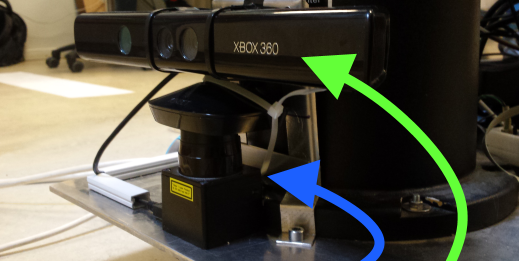
\includegraphics[width=0.85\textwidth]{lidar_and_kinect}
	\caption{Sensor locations for \textcolor{blue}{LIDAR} and \textcolor{green}{Kinect}. }
	\label{fig:kinect_and_lidar}
\end{figure}

\subsection{Sensor Calibration and Setup}

Only support for the Kinect and the \ac{LIDAR} sensor was integrated into this system. Odometry from the two wheel encoders was not included because of time constraints on the project. Figure \ref{fig:sensor_connections} illustrates how the sensors and the wireless router is connected to the \ac{ROS} computer and how they are supplied with power.

\begin{figure}[h]
	\centering
	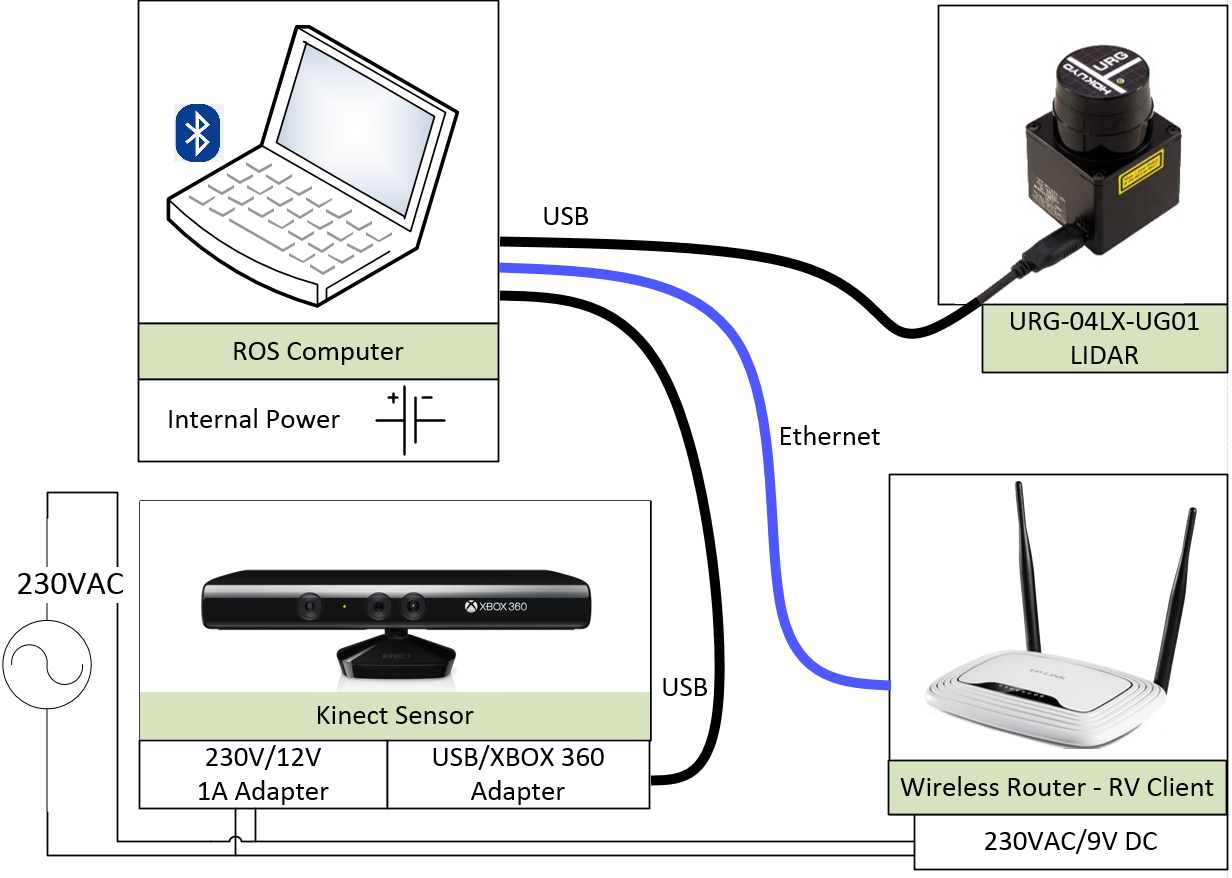
\includegraphics[width=1\textwidth]{sensor_connections}
	\caption{Sensor and power supply connections. }
	\label{fig:sensor_connections}
\end{figure}

Calibrating both the Kinect and the \ac{LIDAR} is a straight forward procedure with \ac{ROS}. The Hokuyo \ac{LIDAR} will in fact be calibrated automatically when the node is launched. Calibrating the Kinect is actually not strictly necessary because the lens distortion is very low. That being said, because there already is a calibration tool available in \ac{ROS}\footnote{ROS calibration guide: \url{http://wiki.ros.org/openni_launch/Tutorials/IntrinsicCalibration}} that is easy to use, there is no good reason to not calibrate. The calibration procedure is as follows:

\begin{enumerate}
	\item Print out a chessboard pattern and tape it to a flat surface. It is beneficial to use A3 paper size to make the pattern easier to detect over a larger set of distances.
	\item Calibrate the RGB camera.
	\item Calibrate the IR camera. It is recommended to cover the IR projector, because the IR speckle pattern makes it difficult to detect the chessboard (figure \ref{fig:ir_calibration}).
\end{enumerate}

The calibration program needs to know the number of inner corners of the chessboard pattern, and the size of the squares. The chessboard used in this project has $6$ by $9$ inner corners and the size of the squares is $0.0275 m$.

 \begin{figure}
 	\centering
 	\begin{subfigure}[b]{0.47\textwidth}
 		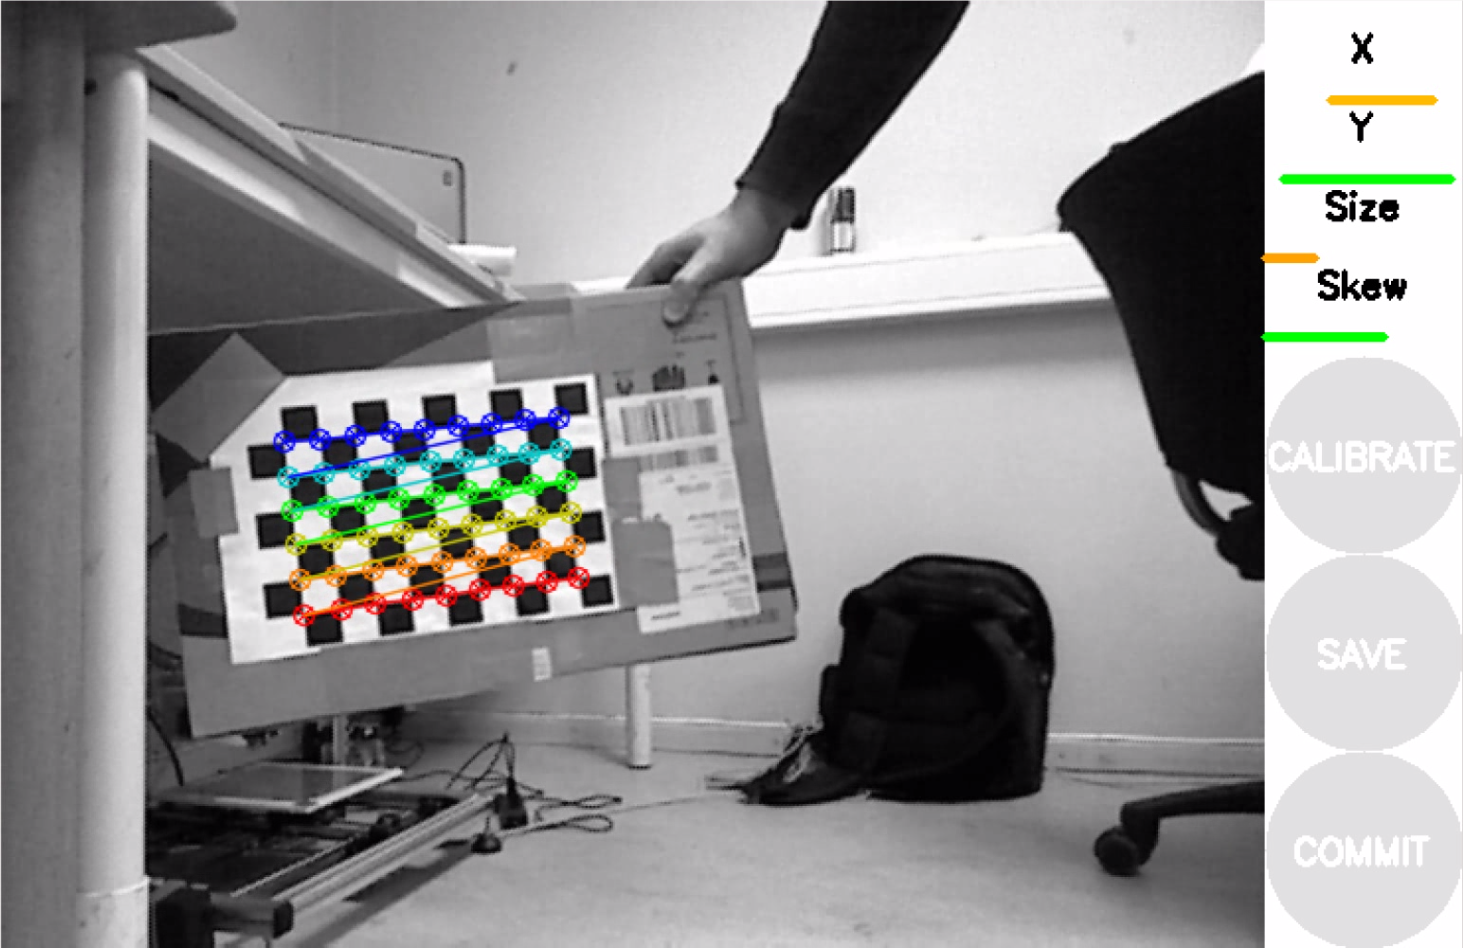
\includegraphics[width=\textwidth]{rgb_calibration}
 		\caption{RGB camera calibration. The camera can be calibrated when a sufficient number of samples have been obtained.}
 		\label{fig:rgb_calibration}
 	\end{subfigure}
 	\begin{subfigure}[b]{0.47\textwidth}
 		
 		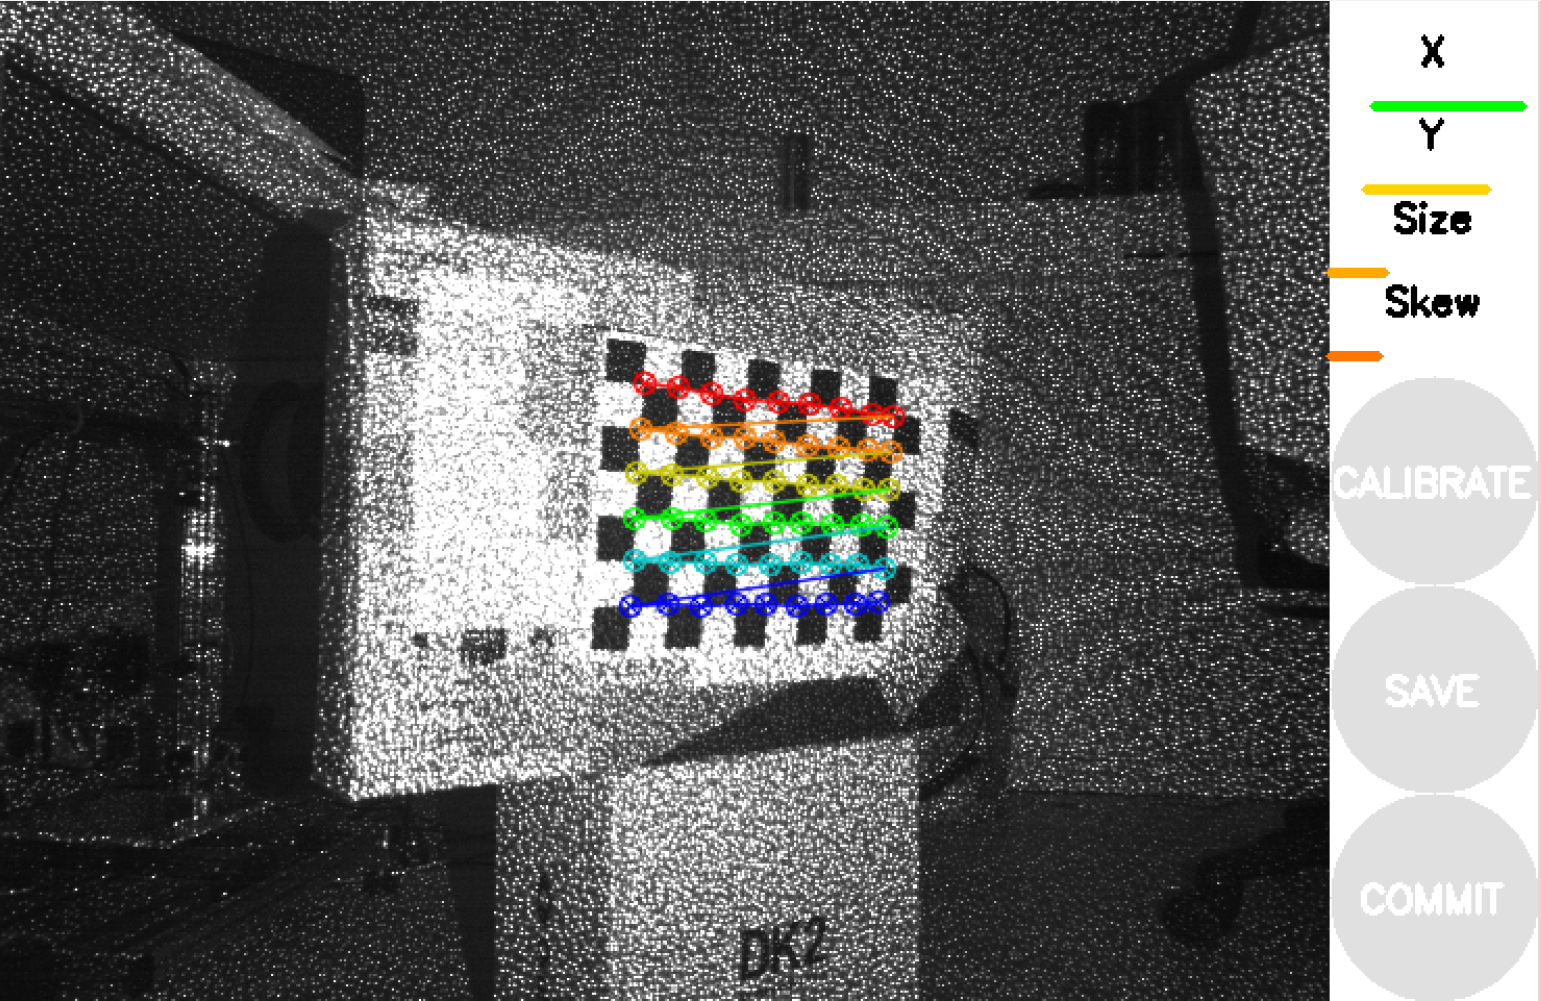
\includegraphics[width=\textwidth]{ir_calibration}
 		\caption{IR camera calibration. The chessboard pattern will be difficult to detect, because the IR projector is not blocked.}
 		\label{fig:ir_calibration}
 	\end{subfigure}
 	\caption{Depth camera calibration.}
 \end{figure}

\subsection{Power Supply and Battery Safety}

\begin{figure}[h]
	\centering
	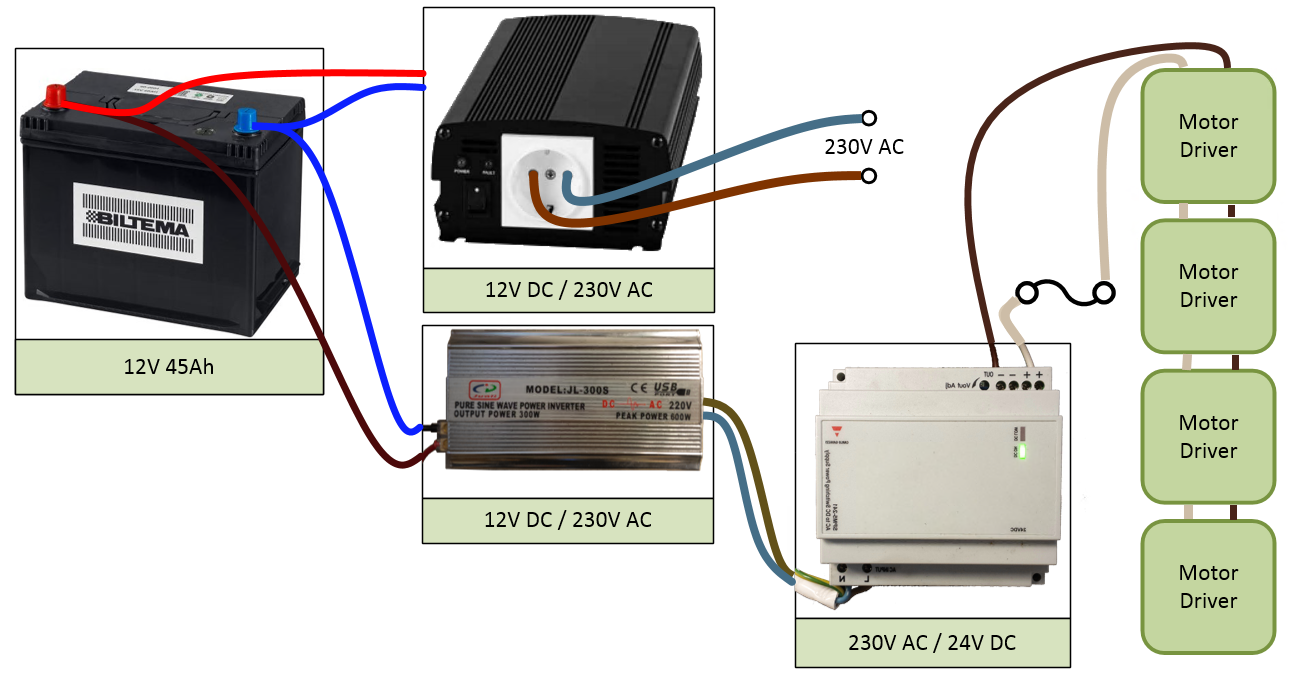
\includegraphics[width=1\textwidth]{power}
	\caption{Example of a feasible power supply setup.}
	\label{fig:power}
\end{figure}

\section{ROS Integration Overview}
\label{sec:integration}
Implementation procedure for mobile robot:

\begin{itemize}

	\item Decide on ROS message interface.
	\item Write interfaces for the motor drivers.
	\item Create a description of the physical structure and properties of the robot in \ac{URDF}. 
	\item Extend the model to enable simulation in Gazebo.
	\item Publish coordinate transform data via \textit{tf} and visualize it in \texttt{rviz}.
	\item Add sensors, with driver and simulation support.
	\item Apply algorithms for navigation and other functionality. 

\end{itemize}

The robot implementation is placed within a \texttt{catkin} workspace (see section \ref{sec:catkin}) that contains all the project specific files that are necessary to build and run the robot system. The overarching file system is shown in figure \ref{fig:file_system}. Note that there are several references to the \ac{TLA} ''mar'', which is short for \ac{MAR}.

\begin{figure}[h]
	\centering
	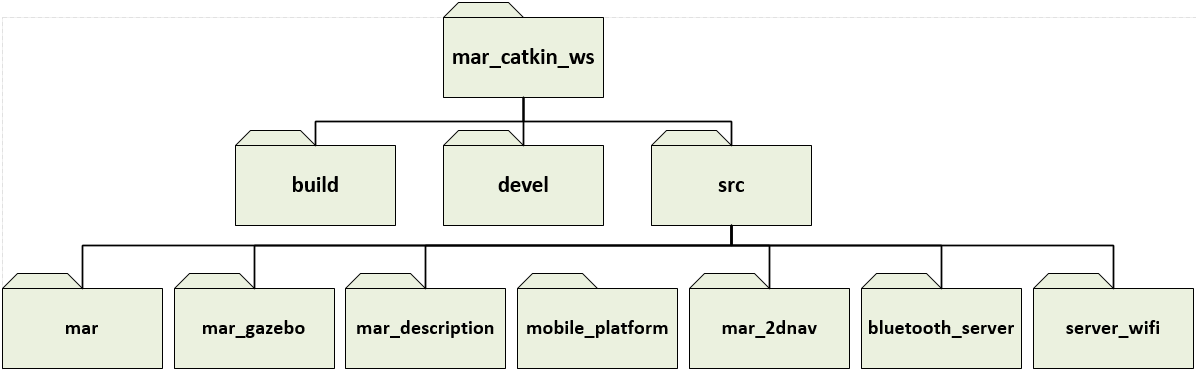
\includegraphics[width=1\textwidth]{file_system}
	\caption{Overarching file system. The \ac{ROS} packages are located within \texttt{src}.}
	\label{fig:file_system}
\end{figure}

Each package will be introduced in the following sections. A short description of each package is given in table \ref{tab:list_packages}.

\begin{table}
	\centering
	\begin{tabular}{ r p{8.5cm} }
		\hline
		\multicolumn{2}{c}{Packages within \texttt{mar\_catkin\_workspace}}\\
		\hline
		\texttt{mar} & Launch files for the real robot hardware and for \ac{RTAB-Map}.\\
		\texttt{mar\_gazebo} & Launch files for the simulated robot and for \ac{RTAB-Map}.\\
		\texttt{mar\_description} & \ac{URDF} files for both the simulated and the real robot.\\
		\texttt{mobile\_platform} & Programs for handling and processing velocity commands. One such node serves as an interface to the motor control card.\\
		\texttt{mar\_2dnav} & Configuration and launch files for both the real and simulated robot.\\
		\texttt{bluetooth\_server} & A node that serves as a Bluetooth server based on the Qt5 API.\\
		\texttt{server\_wifi} & Contains the node responsible for communicating with the \ac{OCS}.\\
		\hline
	\end{tabular}
	\caption{List of custom made packages.}\label{tab:list_packages}
\end{table}


\section{Modeling}

A robot model will serve two purposes in this implementation. First of all, the system needs a definition of how the sensor input is placed with respect to the \texttt{base\_link}. The origin of \texttt{base\_link} is associated  with a coordinate frame. This frame, and any other frame in \ac{ROS}, is right handed, i.e. the positive $x$ direction is \textit{forwards}, positive $y$ points \textit{left}, and positive $z$ is \textit{up}. The robot pose will be based on the transformation between the world and the \texttt{base\_link} frame. 

The second purpose of the model is simulation. Being able to simulate the robot system has been invaluable throughout this project. The robot model is represented in an XML-based modeling language called \ac{URDF} (Unified Robot Description Format). There are two \textit{.urdf} files within the package \texttt{mar\_description}; one for the simulator and one for the real robot hardware. The following sections presents how these models were defined.


\subsection{Physical Dimensions}

Step one in building the model was to define its geometrical shape. The current model shape consists of several links. Each link is defined as a shape and a size. The links are connected together by joints that define the coordinate transformation between the links. All links were modeled as either cuboids or cylinders, in order to simplify and speed up the modeling process. All joints are static except for the wheels which are continuous joints. For simplicity, the robot arm is modeled by a dummy link with the shape of a cylinder.

\begin{figure}[h]
	\centering
	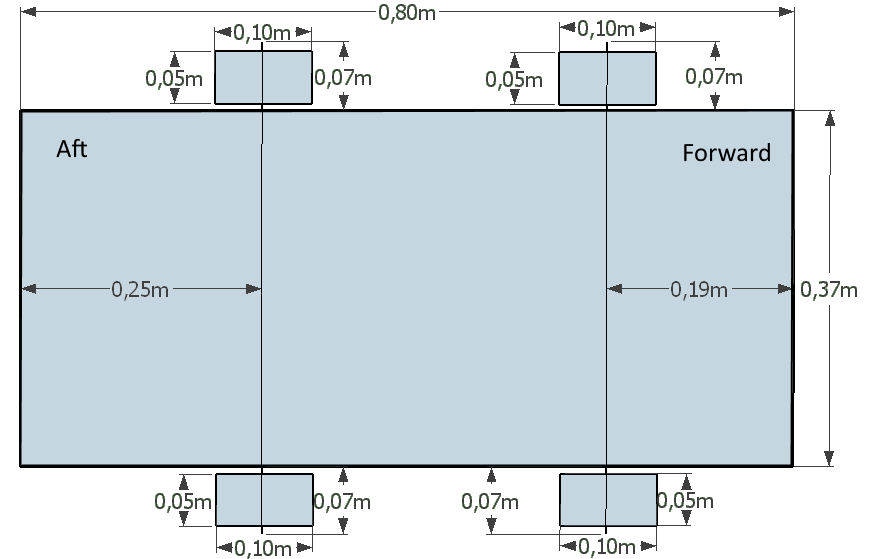
\includegraphics[width=0.85\textwidth]{robotFootprint2}
	\caption{The robot footprint. Dimensions are used for the navigation planners and for modeling. }
	\label{fig:robotFootprint}
\end{figure}

After defining the model shape, it is time to add some additional physical attributes to each link. Each link requires an inertia tensor in order to simulate the model. It is also useful to define a collision volume for each link. In this model, the collision volume is equal to the geometric shape of the link without exceptions. Inertia tensors for each shape is based on equations \ref{eq:cylinder} or \ref{eq:cuboid}.

The inertia tensor:

\begin{equation}
    	I = \begin{bmatrix}
    	I_{xx} & I_{xy} & I_{xz} \\[0.3em]
    	I_{yx} & I_{yy} & I_{yz} \\[0.3em]
    	I_{zx} & I_{zy} & I_{zz}
    	\end{bmatrix}
\end{equation}

Inertia tensor for a solid, uniform cylinder where the radius $r$ is measured in parallel to the $x - y$ plane, and $h$ is parallel to the $z$ axis:
\begin{equation}
I_{cylinder} = \frac{1}{12}m \begin{bmatrix}
	(3 r^2 + h^2) & 0 & 0 \\[0.3em]
	0 & (3 r^2 + h^2) & 0 \\[0.3em]
	0 & 0 & 6r^2
	\end{bmatrix}
	\label{eq:cylinder}
\end{equation}

Inertia tensor for a solid, uniform cuboid. The subscript of $l$ indicates which axis $l$ is measured along:
\begin{equation}
I_{cuboid} = \frac{1}{12}m \begin{bmatrix}
	(l_y^2 + l_z^2) & 0 & 0 \\[0.3em]
	0 & (l_x^2 + l_z^2) & 0 \\[0.3em]
	0 & 0 & (l_x^2 + l_y^2)
\end{bmatrix}
\label{eq:cuboid}
\end{equation}

The mass of each link is guesstimated. Consider the \texttt{base\_link} as an example. The base link was measured to be $5 \; mm$ thick, $37 \; cm$ wide and $80 \; cm$ long. Assuming that the density of aluminium\footnote{https://en.wikipedia.org/wiki/Aluminium} is $2.7 g/cm^3$, the mass of this link was calculated to be $\approx 4 kg$. The base link was defined as follows:

\lstset{language=XML}
\begin{lstlisting}
<link name="base_link">
  <visual>
    <geometry>
      <box size="0.8 0.37 0.005"/>
    </geometry>
    <material name="silver"/>
  </visual>
	  
  <collision>
    <geometry>
      <box size="0.8 0.37 0.005"/>
    </geometry>
  </collision>
	  
  <inertial>
    <mass value="4" />
    <origin xyz="0 0 0" />
    <inertia ixx="0.04564" ixy="0.0" ixz="0.0"
      iyy="0.21334" iyz="0.0" 
      izz="0.25879" />
  </inertial>
</link>
\end{lstlisting}

\subsection{Connecting the Links}

Robot links are connected by joints. A joint defines a translation and rotation from the coordinate frame of a parent link to that of a child link. Each joint has two attributes: \textit{name}, for example ''base\_link\_to\_left\_wheel'' and type, for example ''prismatic'' or ''continuous''. All joints in the mobile robot are static, except for the wheel joints which are continuous. Correct joint transformations is very important when placing the sensors (figure \ref{fig:sensor_frames}). A discrepancy between the real sensor-to-base transform and the modeled transform will cause misaligned sensor input.

 \begin{figure}
 	\centering
 	\begin{subfigure}[b]{0.402\textwidth}
 		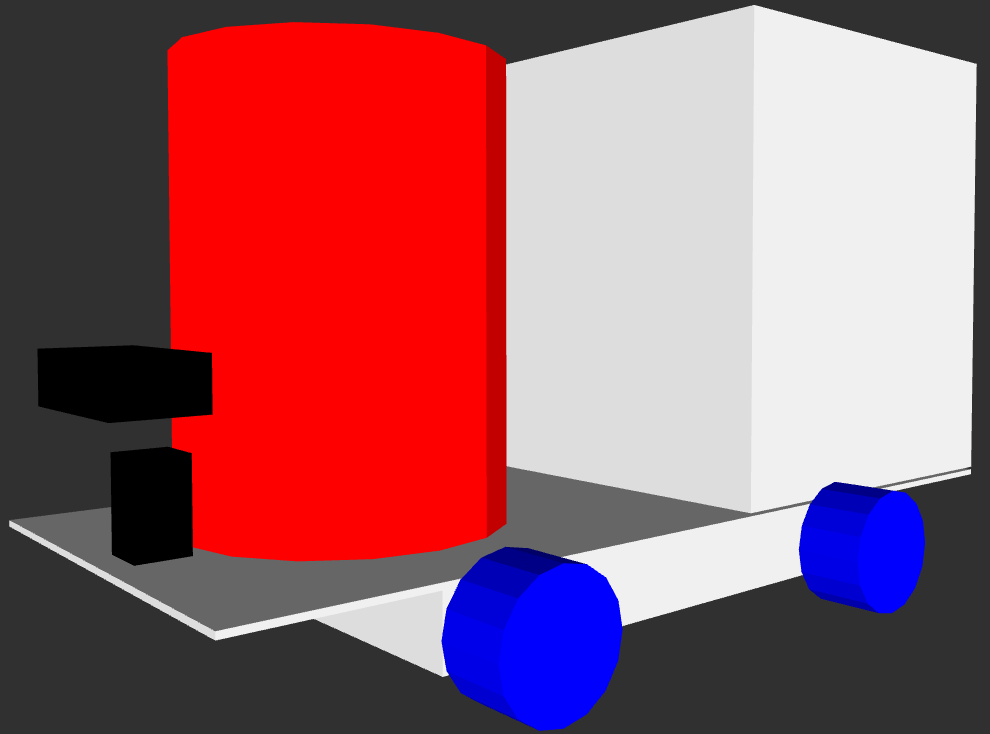
\includegraphics[width=\textwidth]{urdf_model}
 		\caption{Complete \ac{URDF} model when viewed in \texttt{rviz}.}
 		\label{fig:urdf_model}
 	\end{subfigure}
 	\begin{subfigure}[b]{0.51\textwidth}
 		
 		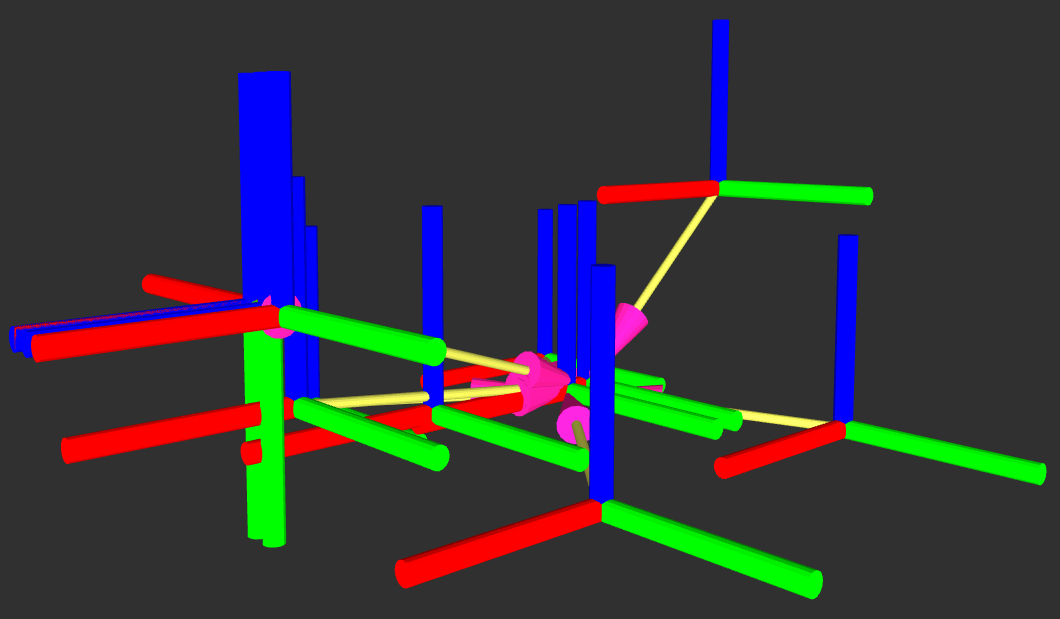
\includegraphics[width=\textwidth]{urdf_tf2}
 		\caption{\ac{URDF} model in \texttt{rviz} with all link frames and transformations.}
 		\label{fig:urdf_tf}
 	\end{subfigure}
 	\caption{}
 \end{figure}

\begin{figure}[h]
	\centering
	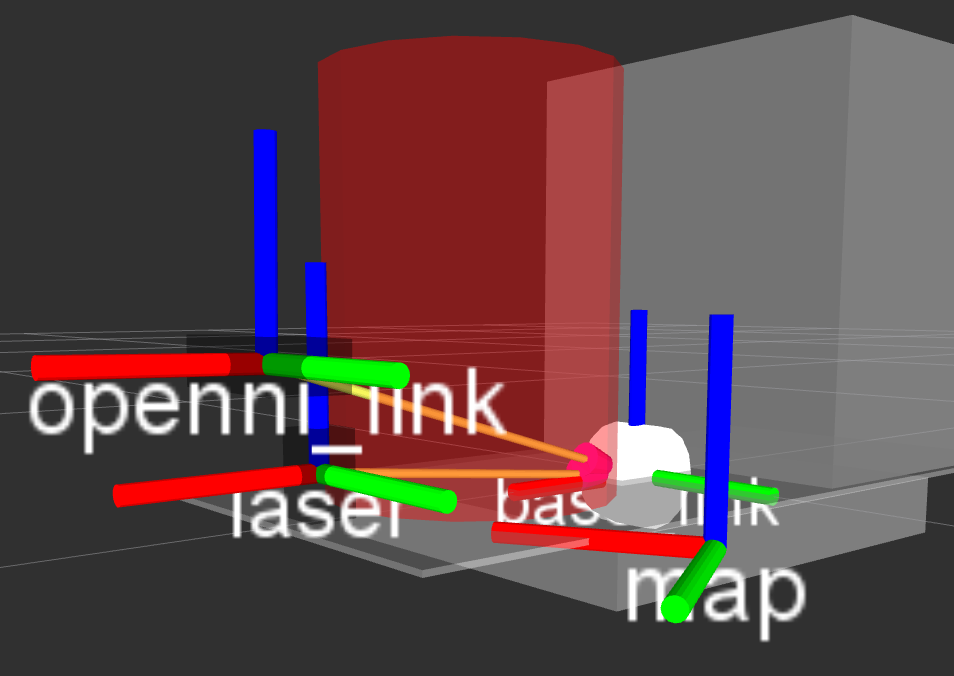
\includegraphics[width=0.5\textwidth]{sensor_frames}
	\caption{Robot model with frames for laser, Kinect, robot base and map. }
	\label{fig:sensor_frames}
\end{figure}

\begin{figure}[h]
	\centering
	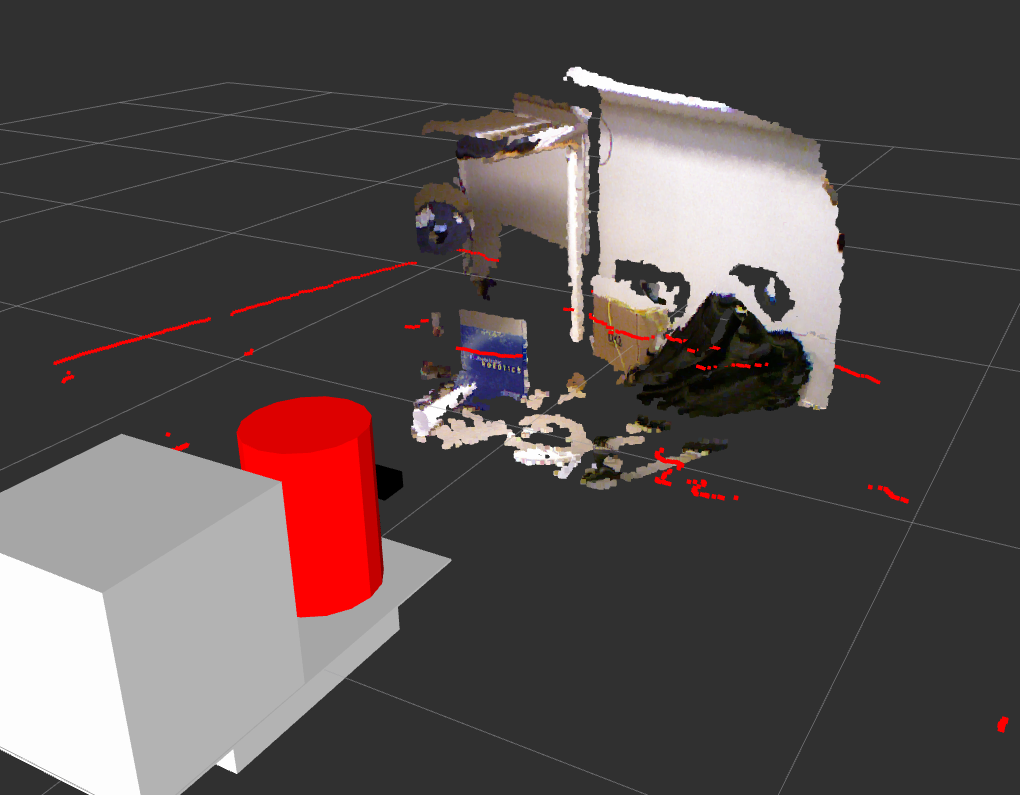
\includegraphics[width=0.5\textwidth]{sensors_in_frame}
	\caption{Sensor input placed with correct transformations from \texttt{base\_link}. }
	\label{fig:sensors_in_frame}
\end{figure}


\section{Simulations}

Robot simulation was done in Gazebo; a simulation tool with good interfaces to \ac{ROS}. The same \ac{ROS} graph was used for both the simulated and real version of the robot, except from the sensors and actuators, and some minor parameter changes. 

\section{Motion Control}

\section{ROS Nodes for Motion Control}


\subsection{Velocity Command Sources}

There are four ways to control the robot:

\begin{itemize}
	\item Local keyboard input.
	\item Wireless teleoperation from the \ac{OCS}.
	\item Wireless teleoperation from a hand-held Bluetooth device.
	\item Commands from the navigation stack in \ac{ROS}.
\end{itemize}

\begin{figure}[h]
	\centering
	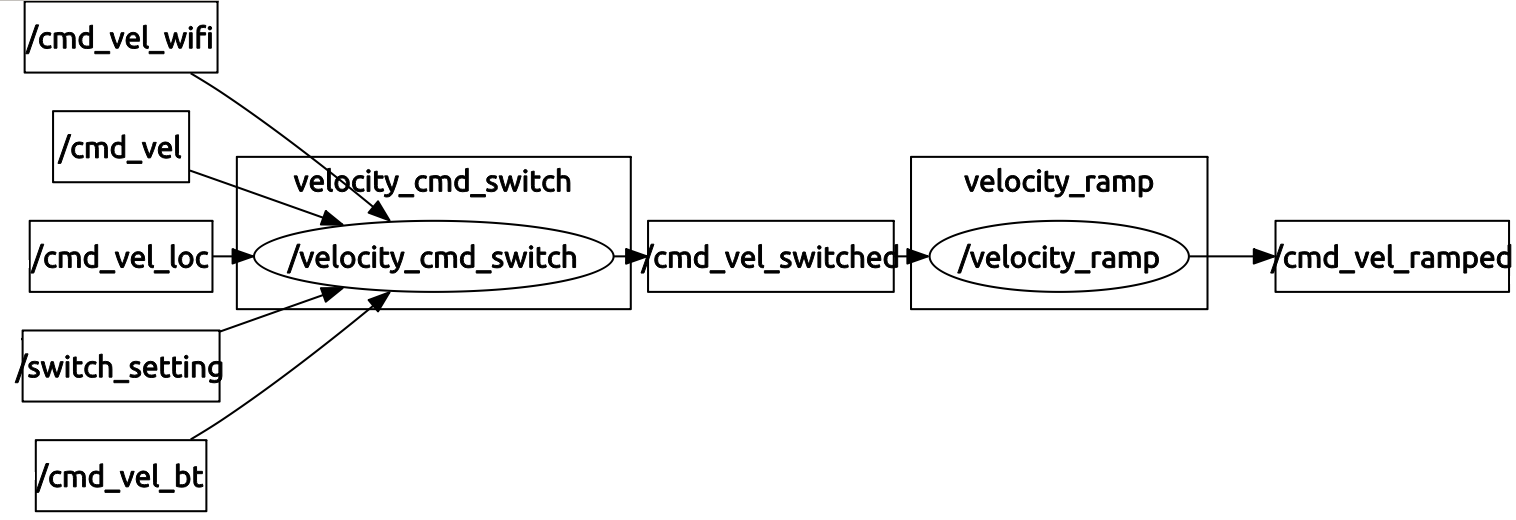
\includegraphics[width=1\textwidth]{velocity_command}
	\caption{Nodes and topics for motion control. (see figure \ref{fig:minimum_graph} for an explanation of this figure)}
	\label{fig:move_base_nodes}
\end{figure}

\begin{figure}[h]
	\centering
	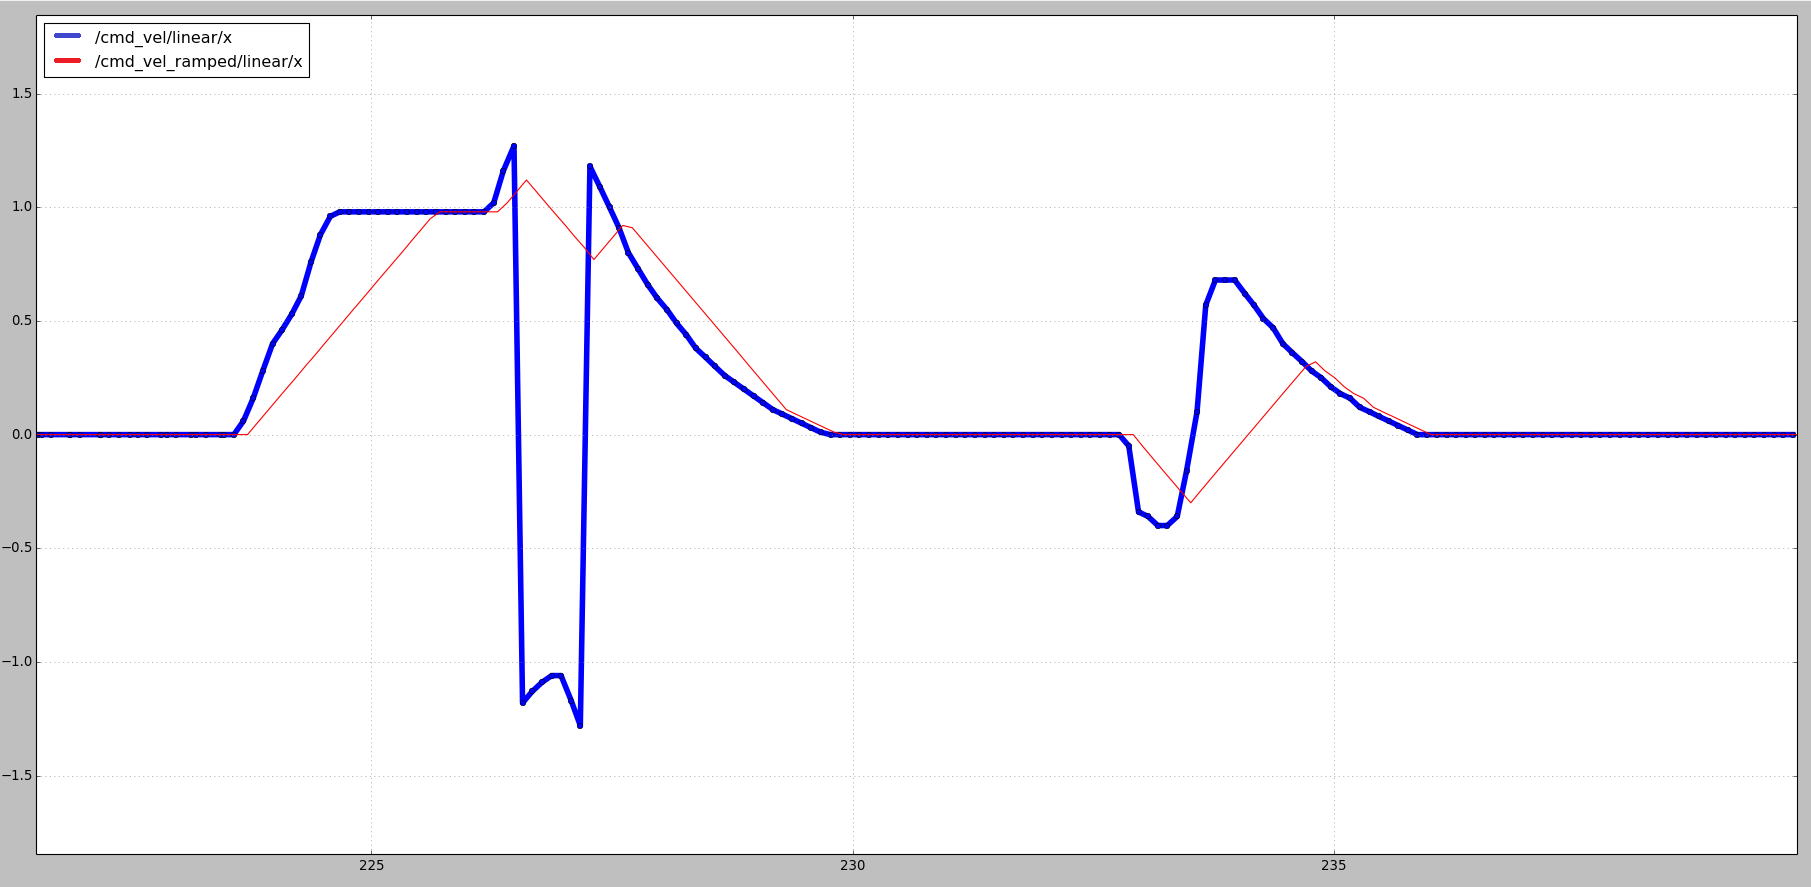
\includegraphics[width=1\textwidth]{velocity_ramp_cropped}
	\caption{Velocity command ramping. The blue line represents commands entering \textit{velocity\_ramp}, while the red line shows the acceleration constrained output command.}
	\label{fig:velocity_ramp}
\end{figure}

\subsection{Motor Control Card Firmware on XMEGA A3BU}

XMEGA A3BU is an evaluation board developed by Atmel. The The implementation presented here is an adaptation of Petter Aspunviks implementation \cite{aspunvik}. The following paragraphs presents the most significant firmware changes that were made.

The firmware will now receive angular and linear velocity commands based on the \texttt{geometry\_msgs/Twist} message format in \ac{ROS}, and translate these into the command format used by each motor. Speed settings for each motor is based on \ac{PWM}. 

There were two requirements for this implementation: 
\begin{enumerate}
\item When velocity commands from the operating system are either absent or incomplete, the robot shall stop.
\item The program shall translate linear and angular velocity commands into wheel commands.
\end{enumerate}

\begin{figure}[h]
	\centering
	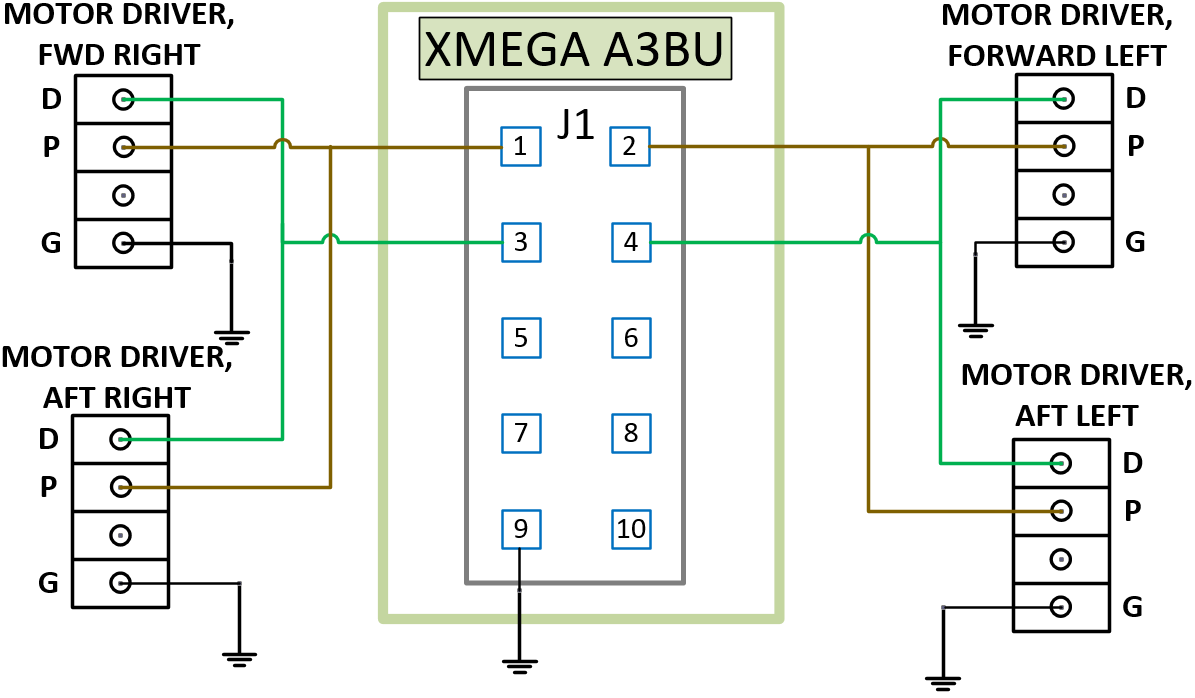
\includegraphics[width=0.9\textwidth]{conn_diag_motors}
	\caption{Connections between each wheel motor driver and the motor control card, XMEGA A3BU. The connections are unchanged from \cite{aspunvik}, except for some improved connection for better short circuit prevention.}
	\label{fig:conn_diag_motors}
\end{figure}

The connections in figure \ref{fig:conn_diag_motors} are the same as in \cite{aspunvik}, except for the installation of more secure connections under the robot. The old connections were insecure, and the risk of short circuits was substantial.

\subsubsection{ROS-Motor Driver Communication}

\begin{figure}[h]
	\centering
	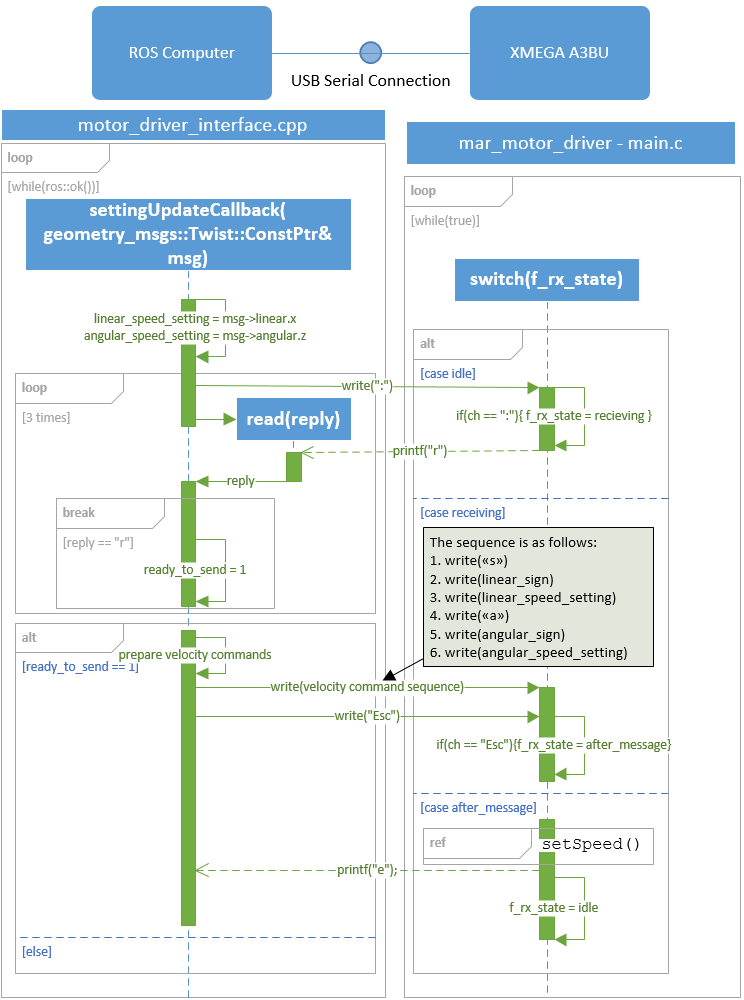
\includegraphics[width=1\textwidth]{motor_cmd_sequence}
	\caption{Velocity command transmission sequence from the \texttt{motor\_driver\_interface} in the ROS computer to the motor control card (XMEGA A3BU).}
	\label{fig:motor_cmd_sequence}
\end{figure}


\subsubsection{From Velocity Commands to Wheel Commands}

Within \ac{ROS}, velocity commands are passed around between nodes in the form of the message \texttt{geometry\_msgs/Twist}. This message type can be viewed as a \textit{struct} with the following contents:

\begin{verbatim}
	Vector3  linear
	Vector3  angular
\end{verbatim}

where each vector contains float values for the directions $x$, $y$ and $z$ with respect to the robot's base frame. Because of the motion constraints of this robot, only \texttt{linear.x} and \texttt{angular.z} are of relevance, and the data which is passed to the motor control card (XMEGA A3BU) is therefore limited to these two values. The motor control card must now translate the linear and angular velocities into wheel speeds. Next, these speeds must be related to a duty cycle for the \ac{PWM} signal which controls each of the four motors.

To perform the translation, it is assumed that the mobile base can be described as a vehicle with differential drive steering. Wheel commands will only distinguish between left or right - not front or aft. Equations of motion which relates angular and linear velocity to wheel velocities can be found in\cite{cook2011mobile}. 

\begin{subequations}\label{eq:subeqns}
  	\begin{align}
	  	\omega &= \dot{\psi} \\
	   	v_{left} &= \omega (R - W/2)\\
	   	v_{right} &= \omega (R + W/2) \label{eq:subeq2}
   	\end{align}
\end{subequations}

$W$ is the spacing between the wheels as shown in figure \ref{fig:robot_kinematics}. In \cite{cook2011mobile}, the parameter $R$ represents the instantaneous radius of curvature of the robot trajectory. This mouthful will be substituted by the linear velocity $v$ in the following equations, because $v = R\omega$ (similar to the linear speed of a wheel). This yields two equations for the wheel speeds, $v_{left}$ and $v_{right}$, based on angular and linear velocity, $w$ and $v$.

 \begin{subequations}%\label{eq:subeqns}
 	\begin{align}
 	v &= R\omega \\
 	v_{left} &=  \frac{2v - \omega W}{2}\\
 	v_{right} &= \frac{2v - \omega W}{2} %\label{eq:subeq2}
 	\end{align}
 \end{subequations}



 \begin{figure}
 	\centering
 	\begin{subfigure}[b]{0.58\textwidth}
 		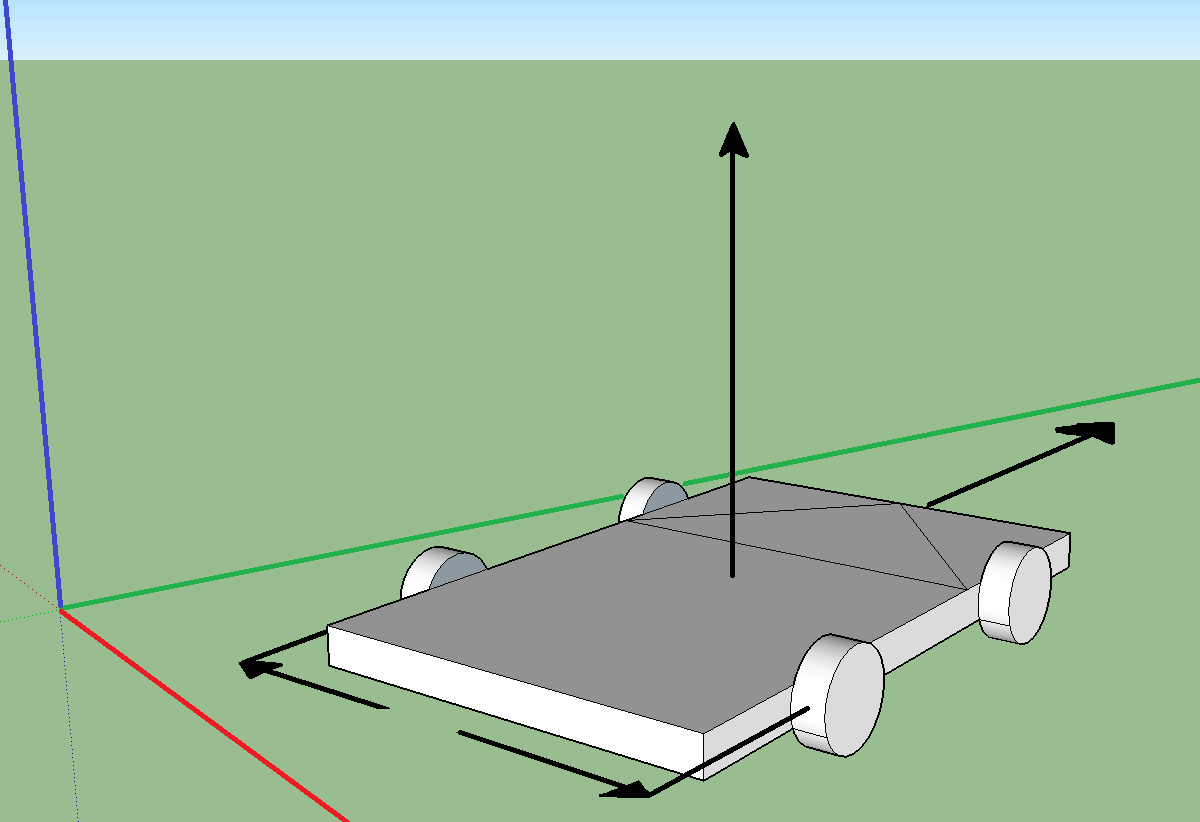
\includegraphics[width=\textwidth]{robot_kinematics}
 		\caption{Differential drive parameters.}
 		\label{fig:robot_kinematics}
 	\end{subfigure}
 	\begin{subfigure}[b]{0.38\textwidth}
 		
 		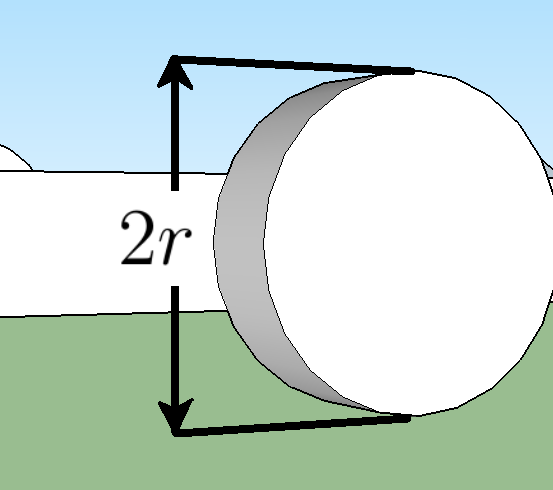
\includegraphics[width=\textwidth]{wheel_diameter}
 		\caption{Wheel diameter.}
 		\label{fig:wheel_diameter}
 	\end{subfigure}
 	\caption{\label{fig:robot_kinematics}Parameters for differential drive kinematics. Note that the frame vectors $\vec{z}$ and $\vec{x}$ refer to the base frame of the robot in this case, and not the world frame.}
 \end{figure}

\section{Operator Control Station (OCS)}

The \ac{OCS} allows an operator to control and monitor the robot through a graphical user interface. \texttt{MainWindow}

\subsection{Graphical User Interface}

A Qt-based \ac{GUI}...

\section{The Hand Held Remote Control - \textit{Robot Leash}}

Because the \ac{OCS} is only partially implemented, an operator will not have access to all the features on the robot. In addition, as a safety precaution a person should be close to the robot at all times, and be ready to pull the plug. Furthermore, it is hard to control a moving robot through the on-board keyboard. These problems were countered by the Android-based remote control, \textit{Robot Leash}. 


\begin{figure}
	\centering
	\begin{subfigure}[b]{0.30\textwidth}
		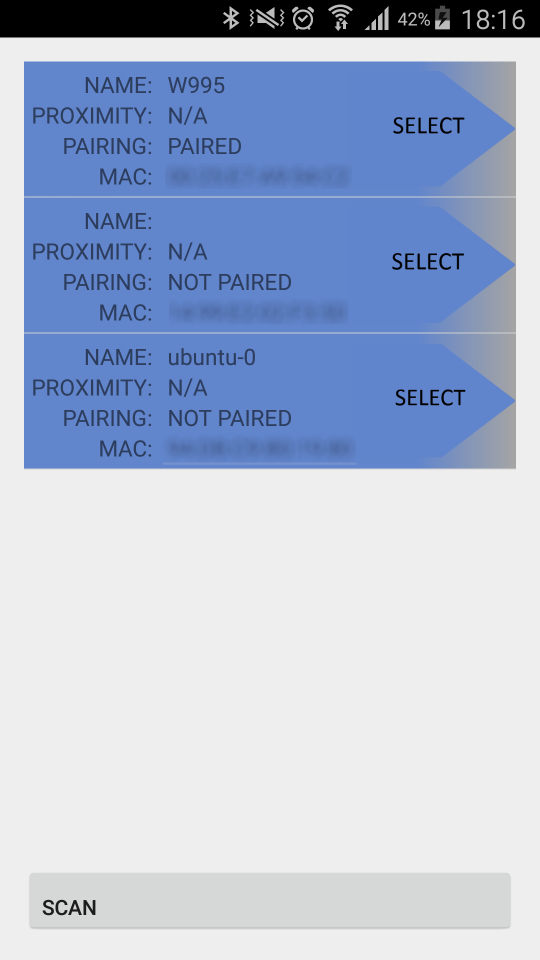
\includegraphics[width=\textwidth]{device_select}
		\caption{First activity with device list.}
		\label{fig:device_select}
	\end{subfigure}
		\begin{subfigure}[b]{0.30\textwidth}
			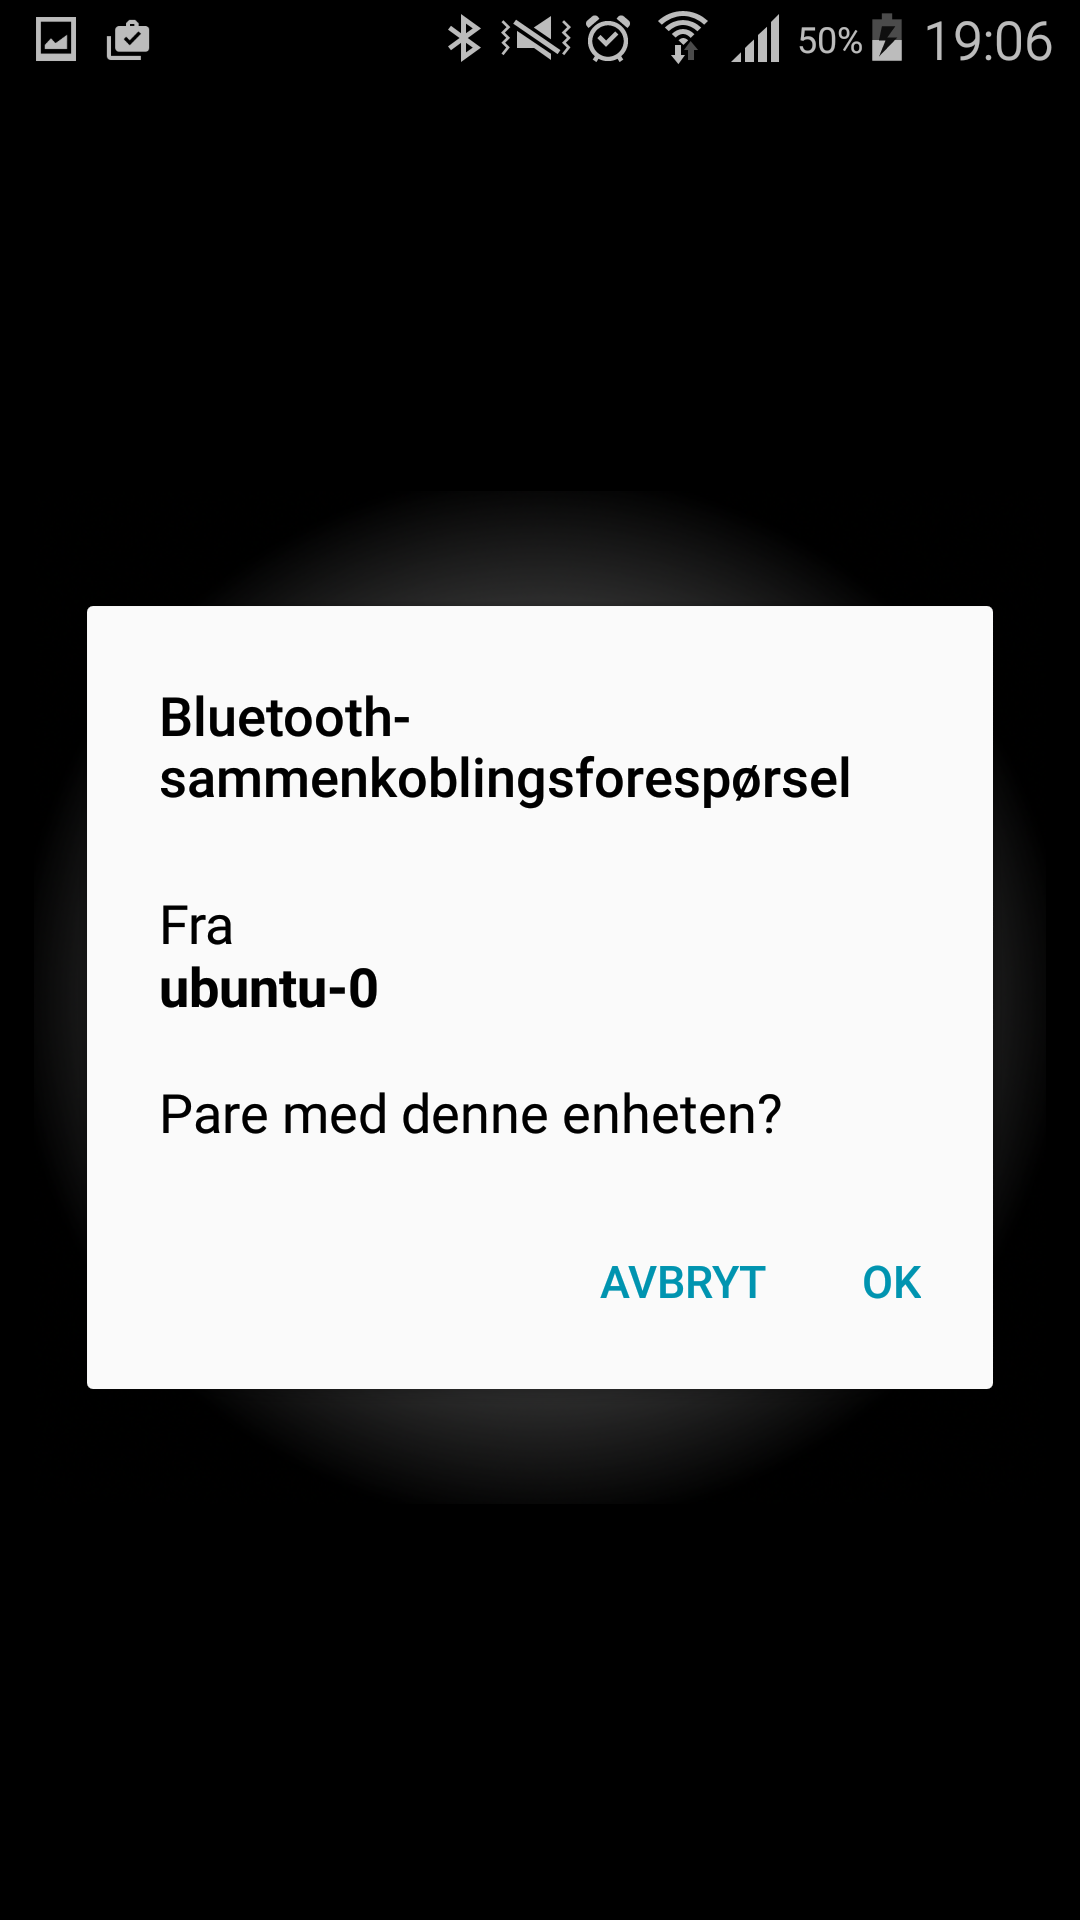
\includegraphics[width=\textwidth]{bt_request}
			\caption{The user is prompted to pair with the robot.}
			\label{fig:bt_request}
		\end{subfigure}
	\begin{subfigure}[b]{0.30\textwidth}
		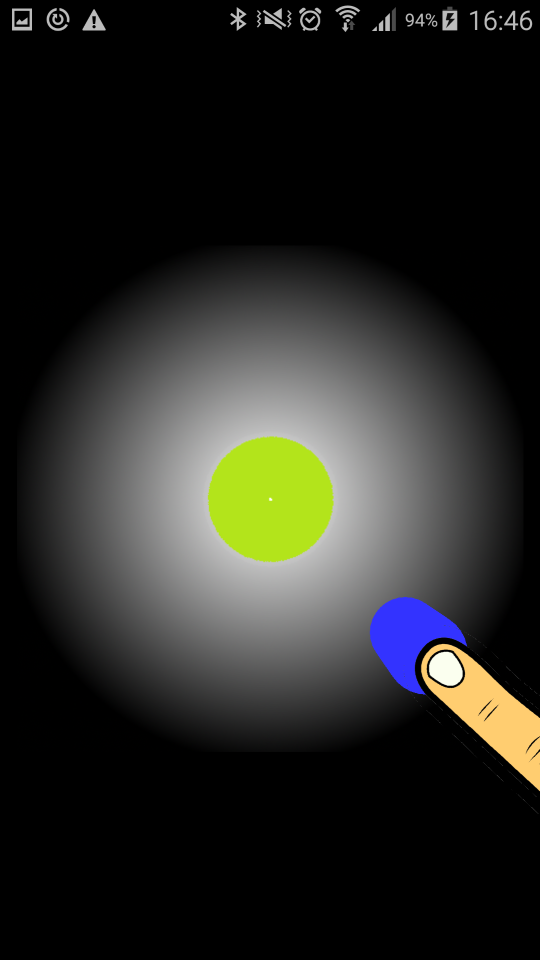
\includegraphics[width=\textwidth]{using_app}
		\caption{Controlling the robot with the stick.}
		\label{fig:using_app}
	\end{subfigure}
	\caption{\label{fig:app_screens}A typical use case for ''Robot Leash''.}
\end{figure}

\subsection{Connecting to the Robot}

\begin{enumerate}
	\item The first screen after scanning for devices. There is no device filtering, and the user can select any device, but only connect through a specific service.
	\item After selecting a device which provides the correct service, the user will be prompted to pair the devices.
	\item The smartphone and the robot is now paired, and velocity commands from the blue control stick are passed to the robot via Bluetooth.
\end{enumerate}

http://developer.samsung.com/technical-doc/view.do?v=T000000117

\begin{sidewaysfigure}[ht]
	\centering
	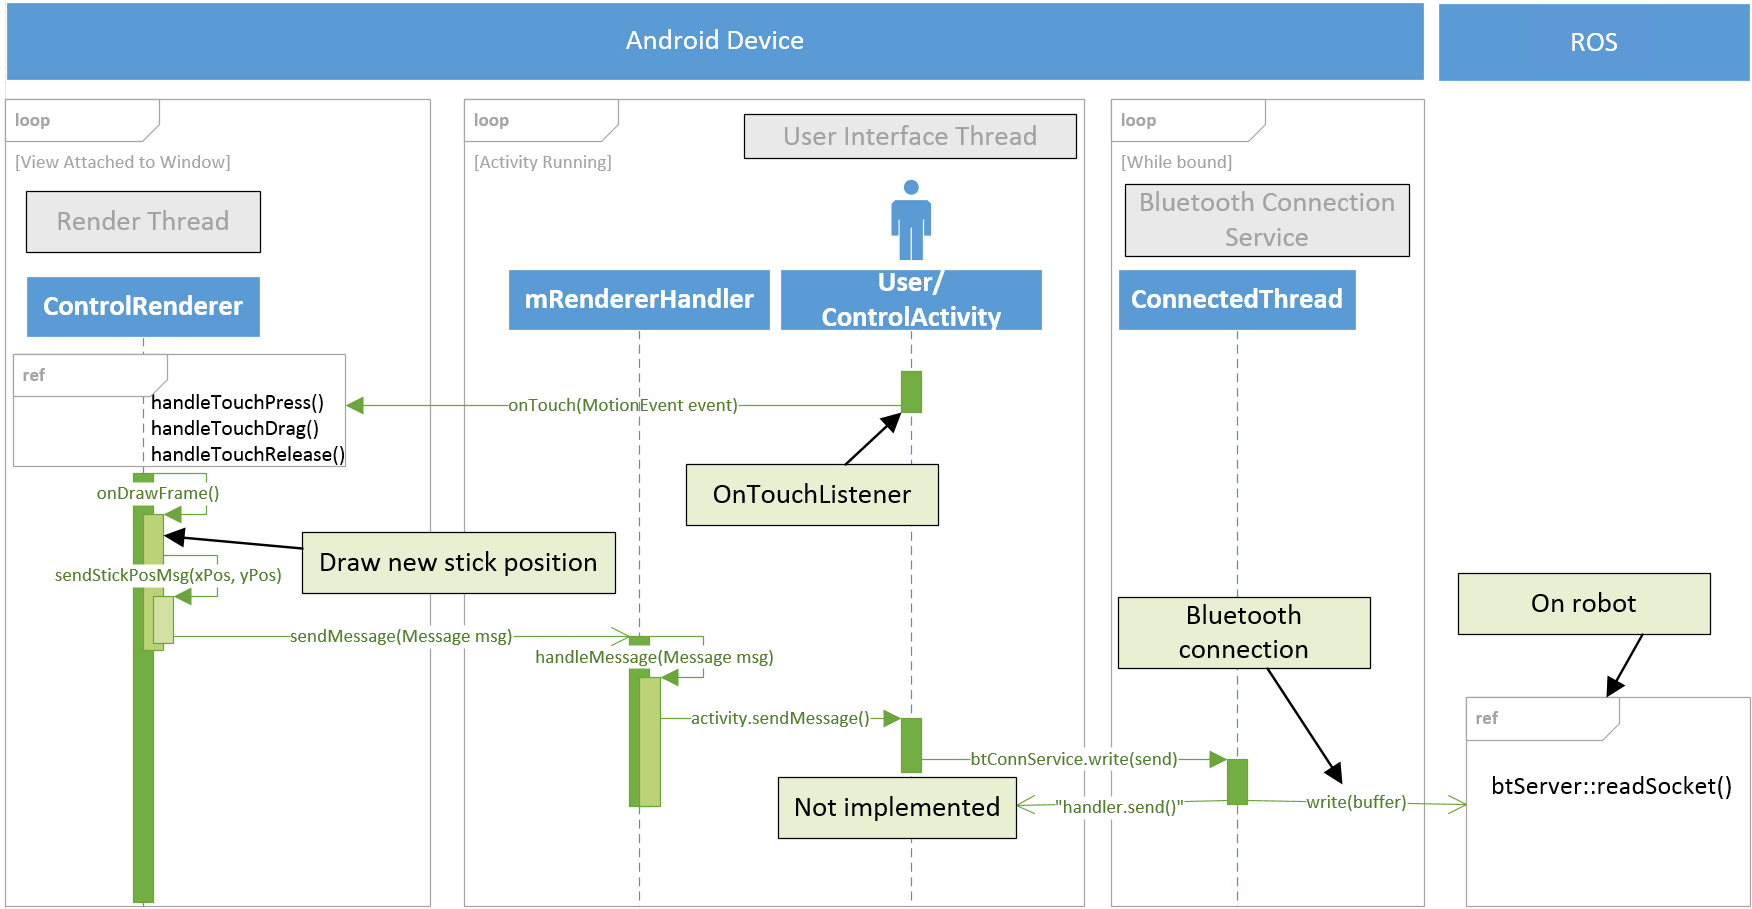
\includegraphics[width=1\textwidth]{android_sequence}
	\caption[This is the caption \newline This is the second line]{\begin{minipage}[t]{.8\linewidth}Sequence diagram illustrating how user touch gestures are detected and propagated \\through the application, before being transmitted as commands to the robot. \end{minipage}}
	\label{fig:android_sequence}
\end{sidewaysfigure}


\section{Mapping - Setting Up RTAB-Map}

For mapping, this robot has utilized Real-Time Appearence Based Mapping (\ac{RTAB-Map}), which was introduced in section \ref{sec:RTAB-Map}. As mentioned, \ac{RTAB-Map} itself has been developed over the last decade by IntRoLab at Université de Sherbrooke in Canada. This section presents how \ac{RTAB-Map} was configured for this robot.

\subsection{Configuration}
\label{sec:configuration}
As all \ac{ROS} programs which are a part of the robot system, \ac{RTAB-Map} will run as a node that subscribes and publishes topics. The first task in configuring \ac{RTAB-Map} is to connect the robots sensor data to the \ac{RTAB-Map} node. The node, called \texttt{rtabmap}, can build 2d occupancy grids and/or 3d point cloud representations of the environment. In this project, \ac{RTAB-Map} is configured to do both. The configuration is based on a guide provided by the developers\cite{rtabmap_setup}. To perform \ac{SLAM}, the mapping node subscribes to odometry, 2D laser scans and camera information. There are five possible sensor configurations with the Kinect\cite{rtabmap_setup}:

\subsubsection{1 - Kinect + LIDAR + Odometry} 
Sensor data can be sent directly to \texttt{rtabmap}.

\subsubsection{2 - Kinect + Odometry + Fake 2D laser from Kinect}

2D laser scans are generated by passing depth images from the Kinect through the node \texttt{depthimage\_to\_laserscan}.

\subsubsection{3 - Kinect + LIDAR}

This is the configuration that was used in this project. Odometry data is generated by a scanmatcher 

\subsubsection{4 - Kinect + Odometry}

This configuration is suitable for uneven surfaces, i.e. when the vehicle is not constrained to a plane. Supports \textit{roll}, \textit{pitch} and \textit{yaw} rotations.

\subsubsection{5 - Kinect}

2D laser scans are generated by passing depth images from the Kinect to the node \texttt{depthimage\_to\_laserscan}.

\begin{center}
	\begin{tabular}{ l p{7cm} }
		\textbf{Kinect + LIDAR + Odometry} & Sensor data can be sent directly to \texttt{rtabmap}.\\
		\textbf{Kinect + Odometry + Fake 2D laser from Kinect} & 2D laser scans are generated by passing depth images from the Kinect to the node \texttt{depthimage\_to\_laserscan}.\\
		\textbf{Android Application} & A supporting tool intended to function as a remote control for the robot. The implementation presented here enables the user to control the robot from an Android device via a Bluetooth connection.\\
		\textbf{Operator Control Station} & A simple Operator Control Station (OCS) based on Qt enables an operator to control the robot via a wireless TCP/IP connection. The \ac{OCS} can display a live video stream from the Kinect sensor. \\
	\end{tabular}
\end{center}

\section{Navigation}

\begin{figure}[h]
	\centering
	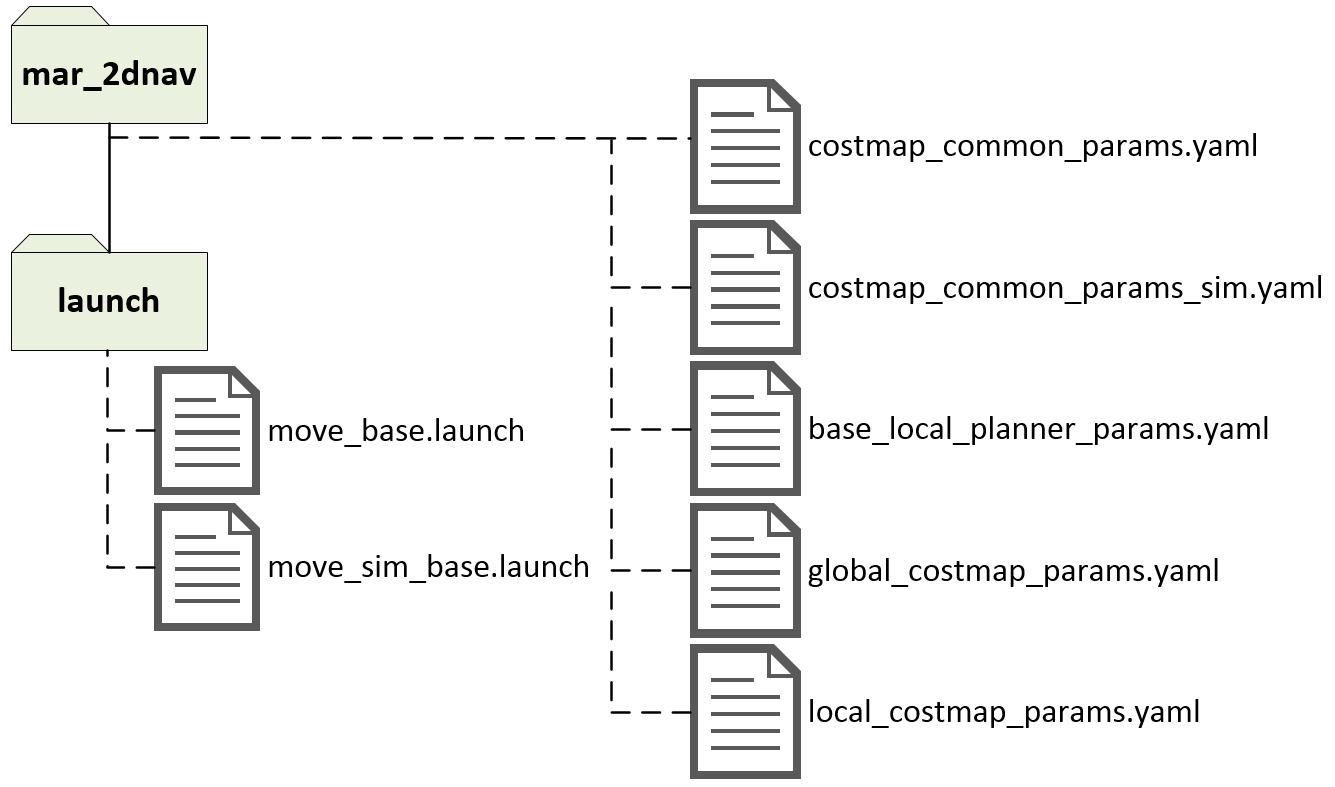
\includegraphics[width=1\textwidth]{mar_2dnav}
	\caption{Files for configuring and launching the navigation stack.}
	\label{fig:mar_2dnav}
\end{figure}

\subsection{Global Path Planning}

\subsection{Local Path Planning}

\subsubsection{Obstruction Detection}

\begin{figure}
	\centering
	\begin{subfigure}[b]{0.53\textwidth}
		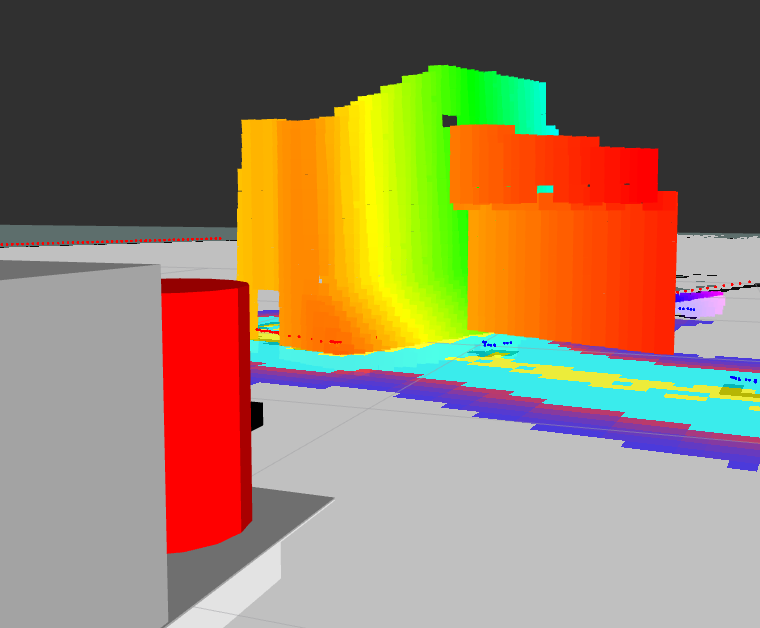
\includegraphics[width=\textwidth]{3d_obstruction1_left}
		\caption{A point cloud representation of the obstruction. Notice how the local costmap is based on the detected point cloud.}
		\label{fig:device_select}
	\end{subfigure}
		\begin{subfigure}[b]{0.45\textwidth}
			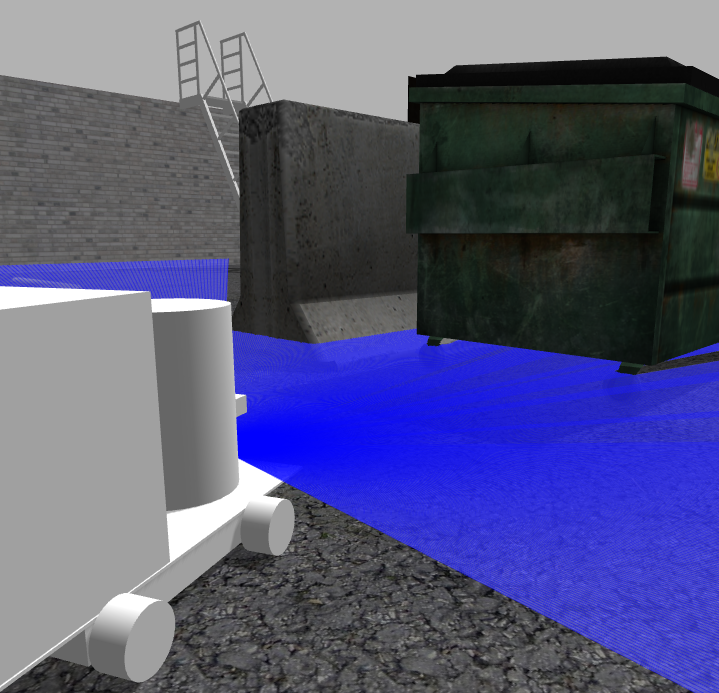
\includegraphics[width=\textwidth]{3d_obstruction1_right}
			\caption{The obstruction in the Gazebo simulator. Notice how the LIDAR only detects the wheels below the container.}
			\label{fig:bt_request}
		\end{subfigure}
	\caption{\label{fig:3d_obstruction1}Detecting obstructions in 3d.}
\end{figure}